%% English translation of effect-systems-free-variables.tex.
%% Standalone article version; build with xelatex + biber:
%%   latexmk -pdf -xelatex effect-systems-free-variables-en.tex
%% (xelatex is used so the < > | glyphs in the code listings render literally,
%%  exactly as in the Russian original; bib.bib is reused verbatim.)
\documentclass[11pt]{article}

\usepackage[a4paper, left=2.4cm, right=2.4cm, top=2.4cm, bottom=2.6cm]{geometry}
\usepackage{fontspec}
\usepackage{amsmath,amssymb,amsfonts}
\usepackage{booktabs}
\usepackage{array}
\usepackage{listings}
\usepackage{tikz}
\usetikzlibrary{positioning, arrows.meta}
\usepackage[english]{babel}
\usepackage{csquotes}
\usepackage{hyperref}
\usepackage[backend=biber, style=numeric, sorting=none, maxbibnames=99]{biblatex}
\addbibresource{bib.bib}
\setcounter{biburlnumpenalty}{9000}
\setcounter{biburllcpenalty}{9000}
\setcounter{biburlucpenalty}{9000}
\AtBeginBibliography{\sloppy}

% --- listings: same lightweight language definitions as the original ---
\lstdefinestyle{modern}{
    basicstyle=\ttfamily\footnotesize,
    keywordstyle=\bfseries,
    commentstyle=\itshape,
    stringstyle=,
    numberstyle=\tiny,
    tabsize=2,
    showspaces=false,
    showstringspaces=false,
    breaklines=true,
    breakatwhitespace=true,
    captionpos=b,
    escapeinside={(*@}{@*)},
    columns=fullflexible,
    keepspaces=true,
}
\lstset{style=modern}
\lstdefinelanguage{colang}{
    keywords={let,var,effect,perform,data,context,fun,where,if,else,throw,try,catch,local,free,op,handle,resume,return},
    sensitive=true, comment=[l]{//}, morecomment=[s]{/*}{*/}, morestring=[b]",
}
\lstdefinelanguage{modal}{
    keywords={fun,let,if,else,handle,with,mask},
    sensitive=true, comment=[l]{//}, morestring=[b]",
}

\title{Effect Systems as a Mechanism for Managing\\ Contextual Free Variables: A Unifying Perspective}
\author{A.\,S. Stoyan\thanks{National Research University Higher School of Economics,
3A Kantemirovskaya Str., Saint Petersburg, 194100, Russia.
Email: \texttt{a.stoyan@hse.ru}. ORCID: 0009-0004-6935-1447.}}
\date{}

\begin{document}
\maketitle

\begin{abstract}
Effect systems lift information about a program's computational effects to the type
level: they sharpen abstraction boundaries and let the compiler verify that an effectful
computation runs in a context that supports it. Nevertheless, static effect tracking has
not yet become common practice: the leading approaches --- effect rows, capabilities, and
modal types --- are usually described using different technical machinery, and a
language designer struggles to see the overall design space. We propose a unifying perspective: an effect
system is a mechanism for managing the contextual free variables of a computation ---
dependencies that are not passed as ordinary arguments but must be resolved by the
execution context. Such a variable goes through a \emph{lifecycle} of two phases: it arises
pending, with an unresolved contextual requirement; once resolved, the dependency can be
retained inside a value --- either literally, by capturing a witness, or more broadly,
as a dependency on its construction context. Families of effect systems differ in
which phases and transitions of this lifecycle they support and how they reflect them in
types. Classical
row-based systems keep the variables pending and
cannot express capture. Capability-based systems allow capture but confine a captured
variable to the context that provided it by means of escape analysis. Modal systems,
instead of forbidding the escape, \emph{uncapture} an escaping variable, re-exposing it in
the type as a contextual requirement. Comparing the families along this single lifecycle axis shows
that the choice of supported transitions predetermines the remaining traits of the
discipline --- from the kind of polymorphism required to the placement of annotations ---
thus giving the language designer a map of the design space.
\end{abstract}

\noindent\textbf{Keywords:} effect systems; computational effects; contextual free variables; free variables; implicit parameters; escape analysis; capabilities; effect rows; modal types; type systems; contextual polymorphism.

\bigskip


\section{Introduction}

Programming is, to a large extent, about managing complexity: a developer strives to
focus on an individual fragment of behaviour without holding the whole program in mind at
once. Abstraction and separation of concerns are the key devices: different
responsibilities are delegated to different entities, such as functions or modules. It is
often convenient to single out, as such an entity, the \emph{execution context} of a
computation, while \emph{effects} arise naturally as the interactions of the computation
with that context~\cite{kiselyov2013extensible}.

Let us start from the opposite notion --- purity. The only observable result of a pure
computation is its value. A function is called pure if it returns the same result given the
same arguments, and its application is a pure computation. Programming with pure
functions is generally considered good practice: the composition of pure functions is
pure, the semantics of the code is transparent, and type systems work well, providing
partial specification, safety, and clarity of abstractions.

However, writing and maintaining a non-trivial program using pure computations alone is
hard. All state and control flow must be managed explicitly through the arguments and
results of functions. Consider an example of manual error propagation --- the function
returns a \lstinline|Result|, and every call is accompanied by a check:

\begin{lstlisting}[language=colang]
    fun readInts(n: Int): Result<List<Int>, Error> {
        if (n == 0) { return Ok(Nil()) }
        let x = readInt()
        if (x is Err) { return x }
        let xs = readInts(n - 1)
        if (xs is Err) { return xs }
        return Ok(Node(x.value, xs.value))
    }
\end{lstlisting}

What is needed is a tool for managing complexity --- something that hides such
inessential details. Computational effects are exactly such a tool. By an effect we
shall mean an interaction of a computation with its execution context; the computation
addresses the context directly, without the ceremony that pervades pure code. The
context may be the run-time system providing OS services, mutable memory cells,
control-transfer mechanisms, input/output, and so on. An \emph{effectful operation} is a
construct that gives rise to an effect. For example, the exception mechanism lets a
computation report an error to the context --- the nearest handler. The routine
propagation of errors disappears from the code --- what remains is the essence:

\noindent\begin{minipage}{\linewidth}
\begin{lstlisting}[language=colang]
    fun readInts(n: Int): List<Int> {
        if (n == 0) { return Nil() }
        return Node(readInt(), readInts(n - 1))
    }
\end{lstlisting}
\end{minipage}

Some approaches let the programmer define their own effects and execution contexts as
library code. In particular, \emph{effect handlers} are a promising approach that has
proved its worth beyond the community of purely functional
languages~\cite{plotkin2013handling, chandrasekaran2018algebraic, phipps2023continuing}.
A handler delimits a scope in which certain effectful operations are admissible, and
interprets them in terms of pure values and the effects of the enclosing scope.
User-defined effects are used to build embedded domain-specific
languages~\cite{leijen2017structured}, and such approaches compete in expressiveness,
performance, and the convenience of composing independently defined
effects~\cite{liang1995monad, kiselyov2013extensible, schrijvers2019monad,
van2024framework}.

Many effectful operations are admissible only within a limited scope. For example, an
exception can be thrown only in the context of a corresponding handler, and a mutable
cell allocated on the stack cannot be used after the function returns. Static control
over the use of such operations prevents many run-time errors and improves program
reliability. \emph{Effect systems} are precisely the mechanism for providing such
control at the type level. Moreover, since effects are inherently implicit at the term
level, their presence is hard to judge from the source code: thus the signature of the
effectful version of \lstinline|readInts| shown above is silent about the possible
error. Some degree of explicitness is therefore still required --- the second task of
effect systems. This helps to state clear functional abstractions and to keep
implementation details from silently leaking as interactions with the context.

The idea of tracking effects in types goes back to the work of Lucassen and
Gifford~\cite{lucassen1988polymorphic} and to the type-and-effect discipline of Talpin
and Jouvelot that developed it~\cite{talpin1994type}; the contrasting trend in the modern
mainstream is equally telling: OCaml~5 has adopted effect handlers without tracking them in
types at all~\cite{sivaramakrishnan2021retrofitting}, which only sharpens the question
of a practical effect system. Many promising effect-system constructions have been
proposed: row-polymorphic types~\cite{leijen2014koka},
capabilities~\cite{brachthauser2022effects, boruch2023capturing}, modal
types~\cite{tang2025modal}, and others. However, each approach has its own strengths and
weaknesses, and the overall picture of the design space remains insufficiently studied.
Yet a language designer needs a holistic view of the available options in order to
choose the most suitable solution given the features and constraints of the target
language.

In this work we propose a unifying view of these seemingly disparate approaches:
\emph{an effect system is a mechanism for managing the contextual free variables of a
computation at the type level}. Such variables are not passed as ordinary term arguments
but must be resolved by the surrounding context: a handler, a resource, or a capability.
This view, which draws on observations from the Scala language~\cite{odersky2021safer,
boruch2023capturing}, lets us regard the classical type system and the effect system as
two sides of one problem: the former deals with variables resolved by the \emph{lexical
environment}, the latter --- with those resolved by the \emph{execution context}. These
variables, in turn, go through a single \emph{lifecycle}, and each of the families of
effect systems under consideration turns out to be a choice of which phases and
transitions of this cycle are available and how they are reflected at the type level.

This paper presents a unifying perspective rather than an exhaustive survey: the scope
is deliberately narrowed to the three leading families. This perspective applies most
directly to effects arising from interaction with the execution context --- such as
exceptions, input/output, or mutable state. The term, however, is also used more
broadly: predicates on computations --- for example, divergence or cost estimates ---
are also called effects; for these, the reading through contextual free variables is
more of an analogy than a literal model.

This work is based on our earlier survey~\cite{stoyan2024modern} but differs from it in
substance. New are the lifecycle model of a contextual free variable itself
(Fig.~\ref{fig:lifecycle}), the notion of \emph{uncapturing} a captured variable, and
the reading of each family in terms of the cycle
(Sections~\ref{sec:rows}--\ref{sec:modal}). Also new are the comparative analysis and
the synthesis (Sections~\ref{sec:comparison} and~\ref{sec:synthesis}).

The contributions of this work can be summarized as follows:
\begin{itemize}
    \item we formulate a single point of view on effect systems as a means of managing
    contextual free variables and describe their \emph{lifecycle}, along whose phases
    and transitions all the constructions under consideration are arranged
    (Section~\ref{sec:idea});
    \item we revisit three families of modern effect systems --- row-based
    (Section~\ref{sec:rows}), capability-based (Section~\ref{sec:capabilities}), and
    modal (Section~\ref{sec:modal}) --- and show which transitions of the cycle each of
    them supports;
    \item we carry out a comparative analysis of the families along a single lifecycle
    axis and show that the choice of supported transitions predetermines both the kind
    of polymorphism required and the placement of annotations, and that the static
    discipline of an effect system, understood as the management of contextual free
    variables, can be regarded as a combination of two mechanisms familiar to
    practitioners --- implicit parameters and type-level escape analysis
    (Sections~\ref{sec:comparison} and~\ref{sec:synthesis}).
\end{itemize}


\section{Free Variables as the Embodiment of Dependencies on the Context}\label{sec:es-intro}

In this section we show that the practical motivation for effect systems arises naturally in
programming practice, and we prepare the ground for the central idea of the work
(Section~\ref{sec:idea}).
Rather than starting from the design of existing systems, we will derive the requirements
for effect systems constructively --- through successive refactorings of an everyday scenario.
For informal explanations we will use examples in a fictional language in the spirit of
Scala and Kotlin, introducing its constructs as needed.

Consider a running example: a business-logic function performs a query to a database. In
the first version it establishes the connection itself:
\begin{lstlisting}[language=colang]
    fun business1() {
        let db = Db.open(...)
        db.query("...")
    }
\end{lstlisting}
This solution has drawbacks. First, the dependency on the database is hard-wired into the
function rather than provided by the context: the calling code cannot vary it --- for
example, replace it in tests. Second, the function produces observable
effects --- accesses to the database --- which are part of its external contract but
are in no way reflected in the signature.

The second version is noticeably better. The function is parameterized by the connection,
and the call site can pass a concrete implementation of it:
\begin{lstlisting}[language=colang]
    fun business2(db: Db) {
        db.query("...")
    }
    fun caller() {
        let db = Db.open(...)
        business2(db)
    }
\end{lstlisting}
Now the behaviour of the function begins to be determined by the execution context, and
the observable effects are explicitly expressed through the parameter \lstinline|db|.
However, this comes at the price of syntactic noise at the call site: the cost of explicit
passing grows with the number of dependencies and the depth of the call stack --- the
parameter is threaded through all intermediate functions, including those that do not use
it. It is precisely this price that inclines developers to look for less cumbersome
solutions.

To eliminate the syntactic noise, in the third version the ordinary parameter is replaced
by a \emph{dynamic free variable} \lstinline|?db|, which obtains its value by lookup in
the dynamic scope of the call:
\begin{lstlisting}[language=colang]
    fun business3() {
        ?db.query("...")
    }
    fun caller() {
        let ?db = Db.open(...)
        business3()
    }
\end{lstlisting}

Nevertheless, the absence of syntactic noise is achieved at the cost of losing other
advantages: the static check of the presence and type of such a variable is lost, as is
the explicit representation of the corresponding effect in the signature.
These losses are made up for by \emph{effect systems}: they offer ways to preserve static
safety without introducing extra ceremony at the term level.
We consider concrete solutions in what follows.

Let us fix the main requirement on an effect system --- \emph{effect safety}: every
effect may be performed only in a context that supports it, otherwise the program must be
rejected. In terms of free variables, this means that every such variable must be
resolved by the enclosing call context.

It is also useful to control what happens to such a variable after it has received a
value. Two events are distinguishable here: first the dynamic variable \lstinline|?db|
is resolved to a concrete value, and then a closure captures that value ---
as a \emph{lexically bound} free variable --- and may outlive the context that
provided it:
\begin{lstlisting}[language=colang]
    fun leak(): () -> Unit {
        let db = ?db // resolution: we obtain the value
        let f =
            () => db.query("...") // lexical capture of the value of db
        return f // the capturing closure leaves leak
    }
\end{lstlisting}
On its own, \lstinline|leak| is not yet unsafe --- everything is decided by the calling code:
if the scope that bound \lstinline|?db| ends before \lstinline|f| is called and, say,
closes the connection, the deferred call will access an already closed connection.

Since many effects are admissible only within a limited scope, such captured variables
must not leak beyond it --- otherwise effect safety would be lost --- and to control
this, an effect system that admits such capture needs some form of escape
analysis~\cite{park1992escape, hannan1998type}. In return, tracking lexical capture makes
it possible not to propagate information about the free variables of an argument function
into the type of a higher-order function --- this technique is called \emph{contextual
polymorphism} and will be considered later (Section~\ref{sec:capabilities}).


\section{The Lifecycle of a Contextual Free Variable}
\label{sec:idea}

The preceding discussion has essentially been about free variables of a special kind.
We will call them \emph{contextual free variables} and understand them broadly: these are
dependencies of a computation on the surrounding execution context
--- an effect handler, a capability value, or a resource, without
which the computation cannot be safely run. The word \enquote{variable} here fixes
not a mandatory syntactic representation but a role in the program: just as a free variable
of a term must be resolved by its environment, so an effectful computation requires support from
the context. We will call the obligation of the context to satisfy such a dependency a
\emph{contextual requirement}.

The central observation of this work is as follows: a contextual free variable may pass through a
\emph{lifecycle} of two phases --- \emph{pending} and \emph{capture}
(Fig.~\ref{fig:lifecycle}). The variable arises \emph{pending}: the body of the function
needs something from the context but has not yet received it; effect systems reflect
such an unresolved requirement in the types. The requirement is then
\emph{resolved} by the surrounding context --- this is how the variable
\lstinline|?db| was resolved in Section~\ref{sec:es-intro}. A deferred computation may preserve the resolved dependency:
literally --- by \emph{capturing} a materialized \emph{witness} value of the
resolution --- or, in
the broad sense, by becoming dependent on the context of its construction.

When a captured variable crosses the boundary of the context that resolved it, a
discipline may respond in two ways: by \emph{confinement} --- forbidding the variable to leave the scope --- or by
\emph{uncapturing} --- moving it back into the pending phase and once more reflecting it in the
type as a contextual requirement\footnote{\enquote{Uncapturing} is the return of the variable
to the status of a \emph{free}, pending one; the term has nothing to do with memory deallocation.}.

Note that \enquote{resolved} is not a separate phase but only an intermediate, locally
resolved state on the transition from pending to capture: the context has already resolved the requirement, but the dependency has not yet
become part of a value capable of outliving the current activation --- such a state needs
no reflection in the types.

The two phases of this cycle correspond to two classical disciplines of \emph{binding} free
variables. A pending variable is, in the characteristic case, bound \emph{dynamically}:
its value (for example, a handler) is determined by the calling context --- although
binding at the definition site is also possible (Section~\ref{sec:rows}). A captured one is bound
\emph{lexically}: the dependency is fixed at the point of capture --- literally by a closure
or, in the broad sense, by the construction context itself.

Let us note a connection with a known notion: an unresolved contextual requirement is, in essence,
a \emph{coeffect} in the sense of works on the context-dependence of computations~\cite{petricek2014coeffects},
whose canonical examples are implicit parameters and dynamic binding.
The orthogonal contribution of the present work is the \emph{capture} layer, with escape analysis and
uncapturing, which coeffect theory does not single out as a separate dimension
(more in Section~\ref{sec:related}).

\begin{figure}[t]
\centering
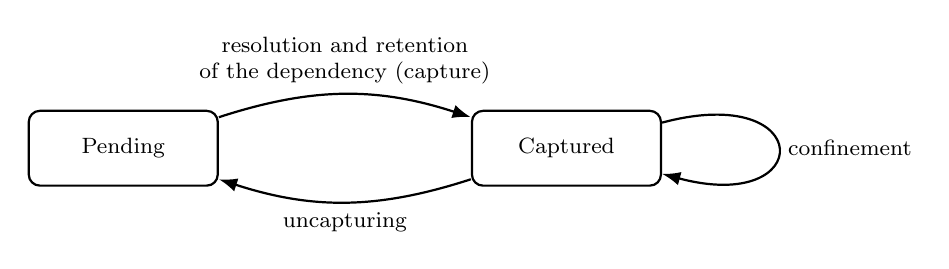
\begin{tikzpicture}[
  node distance=1.0cm and 3.2cm,
  phase/.style={draw, thick, rounded corners, align=center, font=\footnotesize,
                inner sep=4pt, minimum width=2.4cm, minimum height=0.95cm},
  lbl/.style={font=\footnotesize, align=center}]
  \node[phase] (unf) {Pending};
  \node[phase, right=of unf] (cap) {Captured};
  \draw[thick, -{Latex}] (unf) to[bend left=18] node[lbl, above] {resolution and retention\\of the dependency (capture)} (cap);
  \draw[thick, -{Latex}] (cap) to[loop right] node[lbl, right] {confinement} (cap);
  \draw[thick, -{Latex}] (cap) to[bend left=18] node[lbl, below] {uncapturing} (unf);
\end{tikzpicture}
\caption{Lifecycle of a contextual free variable}
\label{fig:lifecycle}
\end{figure}

Let us reiterate once more: we offer a unifying point of view, not a formal
classification and not a proof of the expressive equivalence of all systems.
We stress: we will distinguish the families not by what happens to the variable at
run time, but by which \emph{transitions} of the cycle a discipline supports and how
it reflects them in the types.

In the sections that follow we use this perspective to take a fresh look at the
selected families of effect systems; the comparative upshot --- how the choice of supported
transitions predetermines the shape of the discipline --- is summarized in Section~\ref{sec:comparison},
and the constructive one --- the assembly of a static discipline from the mechanisms of the two phases of the cycle --- in
Section~\ref{sec:synthesis}.


%% NOTE: row-footnote omitted (translation-specific)
\section{Row-Based Effect Systems}
\label{sec:rows}

Most effect systems represent a set of effects by row
types~\cite{gaster1996polymorphic}. This section considers classical row-based
systems, distinguished by storing in the rows information about \emph{all} externally
observable effects of a function. Labels are the names of effects (possibly with type
arguments), and a row is, to a first approximation, an unordered set of labels (its exact
algebra varies from system to system). We will write the row after the result type,
following a slash.

Let us return to the running example from Section~\ref{sec:es-intro}: access to the
database becomes the effect \lstinline|db|, and its label in the row declares the
requirement of the function body:
\begin{lstlisting}[language=colang]
    fun business(): Unit / {db} {
        query("...")
    }
\end{lstlisting}
The operation \lstinline|query|, like the variable \lstinline|?db| before, will be bound
to a concrete implementation from the dynamic call context.

A higher-order function that calls its argument but does not itself satisfy the
argument's contextual requirements produces at least the same effects as the argument
does. Row-based systems express this by \emph{row
polymorphism}~\cite{gaster1996polymorphic}: type variables may denote rows and be
spliced into other rows. Thus \texttt{map} repeats the effect row of its argument via
the variable \texttt{e}:
\begin{lstlisting}[language=colang]
    fun map<e, a, b>(f: (a) -> b / {e}, xs: List<a>): List<b> / {e}
\end{lstlisting}
In general, a higher-order function that calls an argument with effects unknown in
advance and delegates them to the calling context must be parameterized by an
effect-row variable. This substantially hinders a smooth migration to such an effect
system and introduces significant syntactic noise; effect inference (for example, in the
Koka and Flix programming languages) mitigates this burden but does not eliminate row
polymorphism from public signatures.

An example of a row-based system is Java's checked exceptions~\cite{gosling2000java}:
the language statically verifies that all checked exceptions are caught or explicitly
declared in the method signature. This feature has gained a notorious reputation among
programmers~\cite{checked-exceptions}: the exception row is an ad hoc construct that
admits parameterization only by a fixed number of exception variables (generic throws),
not by a variable ranging over an arbitrary set of them, so a higher-order method that
forwards a set of checked exceptions unknown in advance is inexpressible. Fully fledged
rows, in turn, underlie the effect systems of Koka~\cite{leijen2014koka},
Links~\cite{hillerstrom2016liberating}, Flix~\cite{madsen2020polymorphic}, and
Unison~\cite{unison-abilities}.

To satisfy the \lstinline|db| requirement, let us use, for example, an effect handler.
Thus the function \lstinline|withDb| opens a connection, uses it to interpret the
\lstinline|query| operation of the computation passed to it, and closes the connection
upon completion:
\begin{lstlisting}[language=colang]
    fun withDb<e>(f: () -> Unit / {db | e}): Unit / {e} {
        let conn = Db.open(...)
        handle (f()) { op query(s) { resume(conn.exec(s)) } }
        conn.close()
    }

    withDb(() => business())
\end{lstlisting}
The computation \lstinline|f| acts as a client: a call to \lstinline|query| transfers
control to the handler, which executes the query on the open connection and returns the
result to the client by calling \lstinline|resume|\footnote{We regard the effects of
opening and closing the connection as encapsulated inside \lstinline|withDb|: the
signature includes only the requirements on the outer context.}. The signature of
\lstinline|withDb| shows that \lstinline|f| has a set of contextual requirements that
includes \lstinline|db| (the vertical bar extends the row denoted by the variable
\lstinline|e| with this label), whereas \lstinline|withDb| satisfies \lstinline|db| and
delegates the remaining contextual requirements \lstinline|e| to the calling
context\footnote{Note that the handler's scope here deliberately coincides with the
lifetime of the connection: a single lexical scope both resolves the \lstinline|db|
requirement and owns the resource. This coincidence will become essential in the
discussion of leaks (Section~\ref{sec:capabilities}).}.

From the standpoint of the proposed view, a row-based system makes the \emph{pending}
phase explicit. The effect row in a signature is the type-level trace of the pending
contextual variables of the function body that are not yet bound: each label --- such
as \texttt{db} --- denotes an effect that the execution context is obliged to support.
The labels themselves, however, are not term variables but the names of the
corresponding requirements on the context. In lifecycle terms, the call to
\lstinline|query| in the body of \lstinline|f| is an occurrence of a contextual free
variable: the handler dynamically binds it within its scope.

No less important is what this discipline does \emph{not} allow: binding a pending
variable to a value and then capturing it --- such a capture is inexpressible in the
type discipline itself. The association of an operation with a handler is established
anew at each invocation, so the type of a deferred computation continues to enumerate
the variables as pending, into whatever context it may fall. Two consequences follow.
First, row-based systems do not need escape analysis: as long as resolution witnesses
are not materialized in tracked values, a leak is impossible%
\footnote{First-class handler names, which materialize the witness, bring back the need
for scope control (Section~\ref{sec:related}).}.
Second, this is precisely why the volume of annotations grows: a pending variable
cannot \enquote{hide} inside a value, so it has to be repeated in the type of every
intermediate function --- hence the pervasive row polymorphism and the unavailability
of contextual polymorphism.

This association between rows and the dynamic binding discipline also has well-known limits.
First, there exist row-based systems with \emph{lexically} bound handlers: the
association of an operation with a handler is fixed at the point of definition, rather
than by lookup in the dynamic call context~\cite{biernacki2019binders}; handler
tunneling likewise combines the row-based recording with a lexical discipline, solving
the problem of accidental handling~\cite{zhang2016accepting, zhang2020handling}.
Second, the technique of evidence passing compiles Koka's row-based effects into an
explicit passing of handler witness values~\cite{xie2021generalized}. Neither observation
refutes the reading; both refine it. The row says only that the requirement is
still \emph{unresolved}, but does not fix \emph{how} it will be resolved: by lookup in
the dynamic call context, or lexically, at the point of definition. Nor is the requirement's record fixed as a label in the row: evidence passing
systematically turns it into an explicitly passed value --- a handler witness. This
materialization, however, takes place in the compilation target language: to the
source-language programmer the witness is not available as a value, so capture remains
inexpressible in the source discipline. Hence the families differ not in \emph{what}
they track --- it is still the same contextual variable --- but in \emph{how} they
record it. But this choice has a price, and Section~\ref{sec:comparison} will show it:
escape analysis, the kind of polymorphism, the placement of annotations.


\section{Capability-Based Effect Systems}
\label{sec:capabilities}

Previously, effects arose from calls to ``special'' functions --- operations --- and
their labels were listed in row types. Let us now look at effect tracking differently:
suppose effects can be performed only through ``special'' objects ---
\emph{capabilities}, witness values certifying that the context supports the
corresponding effect; the system can then track these objects instead of the operations
themselves.

Let us return to the running example. Passing the connection as an explicit argument
(\lstinline|business2|) is statically safe but noisy; the dynamic variable
\lstinline|?db| is convenient but unsafe. To combine the advantages of both variants, we
approximate the dynamically bound variable by an \emph{implicit parameter} of the
function~\cite{lewis2000implicit}: we declare a group of such parameters with the
\lstinline|context| keyword; a \lstinline|context let| declaration at the call site
makes the value available to the compiler for automatic substitution:
\begin{lstlisting}[language=colang]
    context(db: Db)
    fun business() { db.query("...") }

    fun caller() {
        context let db = Db.open(...)
        business()
    }
\end{lstlisting}
Implicit parameters give types to the contextual free variables of a function: to call
such a function, the context is obliged to supply concrete values --- the very
capabilities\footnote{Implicit passing is a common but not the only option: capabilities
can also be passed as explicit arguments or introduced by handler constructs.}.

Exceptions and other effectful operations are tracked
analogously~\cite{odersky2021safer}: the construct \lstinline|throw SomeException()| can
be understood as a call to a function requiring an implicit parameter of type
\lstinline|CanThrow<SomeException>|, while a \lstinline|try-catch| block provides
witnesses of the corresponding types. Built-in support is not obligatory for this: the
capability discipline is first of all a programming style\footnote{A function does not
reach an effect through a global name or a built-in construct; instead --- like
\lstinline|business2| --- it receives a capability object and calls its methods.},
expressible in Scala with implicit parameters~\cite{odersky2004scala}. The style,
however, rests on convention; built-in exception checking makes it an obligation: the
compiler itself demands a \lstinline|CanThrow| capability at every \lstinline|throw|.

The main new circumstance is that capabilities can be captured by first-class functions.
This gives rise to a lightweight alternative to classical effect polymorphism ---
\emph{contextual polymorphism}~\cite{brachthauser2020effects, brachthauser2022effects}:
the function \texttt{map} can be given its familiar type without any explicit effect
polymorphism --- in contrast to the row-based \texttt{map<e, a, b>}
(Section~\ref{sec:rows}):
\begin{lstlisting}[language=colang]
    fun map<a, b>(f: (a) -> b, xs: List<a>): List<b>
\end{lstlisting}

Unfortunately, for capabilities with a limited lifetime, ensuring safety takes extra
effort: a capability is easily captured by a closure, and the capturing value may
outlive the context that provided it --- that is, leak\footnote{A capability whose
lifetime spans the whole program --- say, a global logger --- may safely escape function calls.}.
For example, if a \lstinline|CanThrow| witness leaves the bounds of its
\lstinline|try-catch| block, the guarantee that all exceptions are handled --- and with
it effect safety (Section~\ref{sec:es-intro}) --- is lost:
\begin{lstlisting}[language=colang]
    fun unsafe() {
        var f
        try { // the capability h: CanThrow<SomeException> is available
            let g = () => throw SomeException() // captures h
            f = g // leak of the computation that captured the capability
        } catch (e: SomeException) { ... }
        f() // throws SomeException outside the handler
    }
\end{lstlisting}
To prevent leaks, escape analysis is needed, and it must be \emph{interprocedural}: the
fate of the capturing closure depends on what the called function does with it. Under
modular checking this behaviour has to be summarized at function boundaries, so the
analysis inevitably leaves a trace in signatures: they state which arguments are used
only in place and which may outlive the call.

Thus \texttt{map} merely applies \lstinline|f| to the elements and does not embed this
function into its result, and escape analysis records this in the signature, for
instance with the \lstinline|local| marker:
\begin{lstlisting}[language=colang]
    fun map<a, b>(local f: (a) -> b, xs: List<a>): List<b>
\end{lstlisting}
It is precisely this non-escaping that lets \lstinline|f| capture capabilities safely:
since it does not leave the call to \texttt{map}, the captured capabilities stay within
the context that provided them\footnote{The \lstinline|local| marker describes the
behaviour of \texttt{map} itself with respect to its argument --- \lstinline|f| is not
retained in its result. It says nothing about captures inside the values that
\lstinline|f| returns: those are reflected independently, in the type \lstinline|b|.}.

The function \lstinline|withDb| from Section~\ref{sec:rows} now takes the following
form --- \lstinline|f| receives an implicit parameter of type \lstinline|Db|, supplied
by \lstinline|withDb|:
\begin{lstlisting}[language=colang]
    fun withDb(local f: context(local Db) () -> Unit): Unit
\end{lstlisting}
The \lstinline|local| marker on the capability \lstinline|Db| is essential:
\lstinline|withDb| closes the connection on completion, so \lstinline|f| is required to
use the capability only in place --- it must not outlive the call either in a closure
that captured it or in a mutable cell (the \lstinline|leak| scenario from
Section~\ref{sec:es-intro} and \lstinline|unsafe| above). The marker on the argument
\lstinline|f| itself is a verdict about the behaviour of \lstinline|withDb|: the
argument is used only in place, which is what allows \lstinline|f| to freely capture
other capabilities from the scope of the \lstinline|withDb| call.

In the proposed perspective, capability-based systems make \emph{both} phases of the
cycle explicit. The pending phase is expressed by the computation's list of implicit
parameters --- the inventory of its contextual requirements: it plays a role close to an
effect row, yet special row types for recording this phase are not obligatory. What is
new is support for the \emph{capture} phase --- exactly the one unavailable to row-based
systems: here the obtained value can be captured by a closure and carried inside a
computation. The confinement of a captured dependency to the scope of the context that
provided it is summarized in signatures by escape-analysis verdicts --- such as the
\lstinline|local| marker.

This has two consequences that explain the shape of the family. First, contextual
polymorphism is a direct consequence of capturing lexically visible capabilities: a
higher-order function need not be polymorphic in effects, because its argument already
carries its own capabilities. Second, the main difficulty becomes not the accounting of
pending variables but \emph{escape analysis}: one must guarantee that a value that
captured a capability does not outlive the scope of the handler or other context that
provided this capability.

The leak ban is realized in different ways, and the approaches differ in the price of
flexibility. The crudest is second-class values: capabilities may not be stored
in freely transferable first-class values --- in particular, into escaping closures,
results, and long-lived mutable cells~\cite{osvald2016gentrification}. Far more flexible
is \emph{lifetime polymorphism}: a captured capability is allowed to get even into the
result, provided the signature states how the lifetime of the result relates to the
lifetimes of the arguments (regions~\cite{tofte1997region}, Rust
lifetimes~\cite{matsakis2014rust}, Scala's experimental capture
sets~\cite{boruch2023capturing}). The price of this flexibility is that these lifetimes
and sets additionally burden the signatures. Related confinement mechanisms are discussed
in Section~\ref{sec:related}.


\section{Modal Effect Systems}
\label{sec:modal}

Capability-based systems made it possible to state in types only a computation's own
requirements, remaining silent about the dependencies already captured by its
arguments. However, they answer leakage with a prohibition
(Section~\ref{sec:capabilities}). Modal systems likewise strive to specify explicitly as
few parts of the context as possible and rely on the same escape analysis, but respond to
a detected leak differently: instead of forbidding it, they uncapture the captured
variable, returning it to the pending phase.

The key idea of the modal notation is to mark the \emph{transitions} between effect
contexts rather than repeat the requirements in the type of every intermediate function.
To this end, the modal system~\cite{tang2025modal} uses two modal type constructors,
parameterized by effect labels; the values of these types are first-class (they may be
stored and passed freely). Computations are boxed with an ascribed modality describing
the required context, and in a suitable context they are automatically unboxed.

The \emph{absolute} modality (square brackets) describes the entire required context.
For example, the familiar \texttt{business} function requires the effect \texttt{db} from
Section~\ref{sec:rows}, while \texttt{map} imposes no constraints on the context:
\begin{lstlisting}[language=modal]
    business : [db](1 -> 1)
    map      : []((a -> b) -> List a -> List b)
\end{lstlisting}
The brackets \texttt{[db]} on \texttt{business} say that running it requires a context
supporting \texttt{db}; the empty brackets \texttt{[]} in the type of \texttt{map} ---
that the body is closed and does not depend on the effect context, so it can be called in
any context; the type \texttt{1} here denotes the unit type.

The \emph{relative} modality (angle brackets) describes relative requirements: a boxed
computation may use both the effects of the surrounding context and those listed in the
type. Its natural habitat is the types of \emph{effect handlers}: a computation passed to
a handler runs under it and can therefore use, on top of the effects of the surrounding
context, the handled ones as well --- exactly what the relative modality describes.
Thus, for the familiar function \lstinline|withDb| (Section~\ref{sec:rows}) the type of
the argument receives a relative modality:
\begin{lstlisting}[language=modal]
    withDb : <db>(1 -> 1) -> 1
\end{lstlisting}
The angle brackets \texttt{<db>} mean that the argument may perform \texttt{db}
\emph{in addition} to the effects of the surrounding context, while \texttt{withDb} itself satisfies this requirement.

The system is built at the junction of two notions: modalities and \emph{kinds}.
The modality ascribed to a boxed
computation expresses its \emph{residual unresolved} requirement on the context.
The kind system, in turn, plays in our perspective the role of escape analysis in a primitive form ---
a coarse binary classification of types by whether their values may depend on the context. Kind $Abs$
is given to types whose values are known not to depend
on the surrounding effect context (such are computations under an absolute modality,
freely transferable between contexts); kind $Any$ --- to types whose values may
carry a captured dependency~\cite{tang2025modal}.
When a value whose type has kind $Any$ is returned from under a handler --- or
otherwise crosses the context boundary --- the system does not reject the program but expresses the captured dependency in
the type by a relative modality, making it explicit again.

Let us demonstrate this on a familiar effect. Suppose that within the scope of the
\texttt{db} handler --- inside \texttt{withDb} --- a function
\texttt{save} is defined that stores data by means of queries.
As long as it is used there, its type is the ordinary \texttt{1 -> 1}, and the dependency
on \texttt{db} remains captured. But if \texttt{save}
leaves the handler's scope (for example, is returned as a result), the result of the
transfer receives a type with a relative modality --- schematically:
\begin{lstlisting}[language=modal]
    save        : 1 -> 1        // inside the db handler's scope
    escapedSave : <db>(1 -> 1)  // the boxed result of the transfer
\end{lstlisting}
The captured variable has become pending again and visible in the type:
\texttt{escapedSave} can now be applied only in a context that supports \texttt{db}.
\texttt{escapedSave} is a modally \emph{boxed} value whose type re-expresses
the dependency of the original \texttt{save} on the context.

From the standpoint of our reading, the modal system works with the same capture phase as
capability-based systems and in essence differs only in its answer to leakage: instead
of simply forbidding a captured contextual variable to leave the context, it
re-exposes it as a requirement on the future context --- traversing the backward edge of
Fig.~\ref{fig:lifecycle}. This transition --- ascribing a relative modality to a value
crossing the boundary, as with \texttt{save}, --- is precisely \emph{uncapturing}
(Section~\ref{sec:idea}): the captured variable returns to the pending phase, and the
type again reflects it as a contextual requirement.

Let us clarify what exactly is captured here: unlike
capabilities, where a closure literally holds a witness value,
the modal system is not obliged to materialize a witness --- the value simply remains
dependent on the context that resolved its requirement. Uncapturing is therefore a
type-level re-abstraction of this dependency, not an extraction of the handler from a
closure at run time. In the Met calculus~\cite{tang2025modal}, a concrete mechanism
corresponds to this reading: the value returned by a handled computation is boxed with
the relative modality of the handled effects by the rules of the system itself --- handler
typing (T-Handler) and return from under it (E-Ret). The term names the abstraction
proposed here over the mechanism of modal types, not a new rule on top of the system.

Thus, here leak control does not reduce to a \emph{prohibition}, as in
Section~\ref{sec:capabilities}: part of the leaks turns into the re-exposure of the
contextual variable in the type. We stress that the prevention of
unsafe leaks does not disappear: it is performed by the same classification by kinds.


\section{Comparative Analysis}
\label{sec:comparison}

Let us bring the three families into a single picture. The proposed point of view reduces the
comparison of the families --- each taken in its characteristic guise --- to two questions about
the lifecycle of a contextual free variable: can a resolved dependency be retained inside a
value --- literally, as a captured witness, or more broadly, as a dependency on its construction
context; and if it can --- what happens when such a value is transferred across the context
boundary. Row-based systems answer \enquote{no} to the first question: a resolved dependency is
not retained in the value, and in the type of a suspended computation the variable remains
pending. Capability-based and modal systems answer \enquote{yes} and diverge on the second: the
former forbid the leak, the latter return the leaked variable to the pending phase. Everything
else --- the very recording of the pending phase, what polymorphism is required, and, in
particular, where the annotations concentrate --- turns out to be a \emph{consequence} of these
answers, not an independent dimension. The comparison is given in Table~\ref{tbl:compare}.

\begin{table}[!tbp]
  \caption{Three families of effect systems along the single lifecycle axis}
  \label{tbl:compare}
  \centering
  \footnotesize
  \begin{tabular}{>{\raggedright\arraybackslash}p{2.6cm}>{\raggedright\arraybackslash}p{3.2cm}>{\raggedright\arraybackslash}p{3.2cm}>{\raggedright\arraybackslash}p{3.6cm}}
  \toprule
  & \textbf{Row-based} & \textbf{Capability-based} & \textbf{Modal} \\
  \midrule
  Explicit phases and transitions & pending (row of labels) & pending (implicit parameters), capture and confinement (escape-analysis verdicts) & pending (modalities), capture and transfer control (escape analysis), uncapturing (relative modality) \\
  Can a resolved dependency be retained in a value? & no: in the type the requirement remains unresolved & yes: by literal capture & yes: as a dependency on the construction context \\
  Polymorphism (a consequence) & row & contextual (via capture); with fine-grained escape analysis --- lifetime & over the enclosing context (via unboxing); effect variables --- in the Met extension \\
  Annotations (a consequence) & in the signatures through which the requirement propagates & in implicit-parameter declarations and escape-analysis verdicts & at the points of transfer between contexts \\
  Ensuring safety & capture inexpressible; running --- only in a context that supports all effects in the row & prohibition of leaks detected by escape analysis & unboxing --- only in a suitable context; a leaked variable returns to pending \\
  Price & pervasive row polymorphism & escape analysis & modalities at transfer points; escape analysis \\
  Example systems & Koka, Links, Java's checked exceptions & Effekt, Scala & Met~\cite{tang2025modal} \\
  \bottomrule
  \end{tabular}
\end{table}

The pattern is visible in the consequence rows of Table~\ref{tbl:compare}: the choice of phases
and transitions determines what polymorphism the discipline \emph{needs} and where its
annotations concentrate. The justification unfolds into a short chain of consequences. If a
resolved dependency cannot hide inside a value, the requirement remains unresolved and is forced
to propagate through the types of the calling computations: hence the special row types and the
pervasive row polymorphism of higher-order functions. If, on the other hand, the dependency can
be retained in a value --- by literally capturing a witness or in the broad sense --- the
requirement hides inside it. This yields contextual polymorphism and dispenses with explicit
effect variables (the pending phase is recorded by the very list of implicit parameters or by
the modality), but makes escape analysis --- control over the transfer of such a value ---
necessary. The analysis itself can be coarser or finer --- from second-class values to lifetime
polymorphism; the discipline, in turn, chooses its response to a detected leak: confinement, or
re-exposing the dependency in the type as a requirement on the receiving context ---
uncapturing. Hence the kind of polymorphism and the principal placement of annotations follow
from how the dependency is represented, how precisely its transfer is controlled, and how the
discipline responds to a leak. Capture, meanwhile, does not forbid polymorphism over sets of
pending variables --- it makes it optional.

Behind the variety of polymorphisms, in turn, stands a common mechanism: in all three families
polymorphism is a way to record in a signature how a call and its result depend on the
arguments, and what differs is only \emph{what} the variable denotes. In rows it denotes a set
of labels --- the names of unresolved requirements; in lifetime polymorphism --- the lifetimes
of captured capabilities or, as in Scala's capture sets, those capabilities themselves. Modal
notation, in its characteristic case, needs no explicit variable at all --- its role is played
by the enclosing context itself; where effect polymorphism is nevertheless needed explicitly, it
is provided by the Met extension with effect variables~\cite{tang2025modal}.

Let us emphasize: the lifecycle is an analytical axis, not a partition of systems into disjoint
classes. Real disciplines combine techniques: there are row-based systems with lexical binding
of handlers (Section~\ref{sec:rows}), evidence passing materializes a row requirement as a
value, ZIO~\cite{zio-lib} combines witnesses with polymorphism over sets of requirements, and
boxing with \texttt{box} in the Effekt language corresponds to the modal notation
(Section~\ref{sec:related}). The table describes the characteristic guise of each family, not
its boundaries.

The running example \texttt{withDb} makes these differences concrete
(Table~\ref{tbl:withdb-three}; the signatures repeat those of
Sections~\ref{sec:rows}--\ref{sec:modal}). In the row-based system the type names everything:
the handled label \texttt{db} in the argument's row and the variable \texttt{e} for the rest of
its effects, which \texttt{withDb} repeats in its own effect row, delegating them to the outer
context. In the capability-based system the handled effect has become an implicit parameter of
type \texttt{Db}, while about the remaining effects of \lstinline|f| the type is silent: they
arrive as captured capabilities --- contextual polymorphism. The silence is paid for by the
\lstinline|local| markers --- escape-analysis verdicts directly in the signature: both the
argument itself and the capability issued to it are used only in place. In the modal system the
handled effect is expressed by the relative modality \texttt{<db>}, and about the remaining
effects the type is silent here as well: the argument may use the effects of the enclosing
context~\cite{tang2025modal}. Neither effect variables nor the \lstinline|local| marker is needed here: the role of the
former is played by the enclosing context, and the admissible contexts for using the
value are already fixed by its relative modality --- once it lands in a suitable one,
under the handler in \texttt{withDb}, it is simply unboxed.

\begin{table}[!tbp]
\caption{The type of \texttt{withDb} across the three families}
\label{tbl:withdb-three}
\centering
\footnotesize
\begin{tabular}{@{}l@{\hspace{6pt}}l@{}}
\toprule
\textbf{Family} & \textbf{Type of \texttt{withDb}} \\
\midrule
Row-based        & \lstinline[language=colang]!fun withDb<e>(f: () -> Unit / {db | e}): Unit / {e}! \\
Capability-based & \lstinline[language=colang]|fun withDb(local f: context(local Db) () -> Unit): Unit| \\
Modal            & \lstinline[language=modal]|withDb : <db>(1 -> 1) -> 1| \\
\bottomrule
\end{tabular}
\end{table}


\section{Synthesis: An Effect System from Two Familiar Parts}
\label{sec:synthesis}

A single axis suggests a constructive programme: the static discipline of an effect
system, understood as the management of contextual free variables, can be designed as a
combination of two independently useful mechanisms already familiar to practitioners ---
\emph{implicit parameters} (for the pending phase) and \emph{type-level escape analysis}
(for the capture phase). The pair does not define the semantics of the effectful
operations and handlers themselves --- it provides a mechanism for their static control.
The recipe mirrors the lifecycle (Fig.~\ref{fig:lifecycle}):
\begin{enumerate}
    \item unresolved requirements are declared as implicit parameters: the function
    \lstinline|business| from Section~\ref{sec:capabilities} does not open the connection
    itself and does not drag it along as an extra argument, but declares
    \lstinline|context(db: Db)|;
    \item binding is performed by the call site, providing the value through
    \lstinline|context let|;
    \item a closure may capture the obtained value --- this gives contextual
    polymorphism --- while escape analysis confines the captured value to the scope of the
    context, and its verdict is visible directly in the signature (the \lstinline|local|
    markers in Table~\ref{tbl:withdb-three});
    \item upon an attempted transfer across the context boundary, the system either
    forbids it (Section~\ref{sec:capabilities}) or performs uncapturing
    (Section~\ref{sec:modal}); note that in the second case, too, determining the place
    where uncapturing must occur requires some form of escape analysis.
\end{enumerate}

In a language that already has implicit parameters, this path may require fewer new
constructs than full-fledged row types: implementations of implicit parameters already
exist~\cite{KEEP-context-parameters, oliveira2010type, lewis2000implicit}. The usefulness
of type-level escape analysis, in turn, extends beyond effect systems: it makes it
possible to reduce interprocedurally the number of heap
allocations~\cite{lorenzen2024oxidizing}, to support such language mechanisms as
ownership-based borrowing in resource
management~\cite{matsakis2014rust, lorenzen2024oxidizing} and non-local
returns from non-escaping lambdas~\cite{akhin2021kotlin}.


\section{Related Work}
\label{sec:related}

The proposed perspective is not the only attempt to bring rows, capabilities, and modal
types under a common view. Below we relate it to other unifying approaches and sketch the
historical lineage.

Closest to our work are Tang and Lindley~\cite{tang2026modal}. They introduce the core
calculus Met(X) --- a generalization of the modal system~\cite{tang2025modal},
parameterized by an effect structure --- and encode into it both Koka's row-based system
(System F$^\epsilon$) and Effekt's capability system (System C), proving that types and
semantics are preserved. They thereby formally confirm that both rows and capabilities
are expressible as modal effects, and along the way arrive at observations close to ours:
a capability acts as an implicit form of parametric polymorphism, and Effekt's
\texttt{box} construct corresponds to the absolute modality. What differs is the axis and
the purpose. Their axis is whether effect tracking is attached to function types: the
row-based and capability-based notations place effects on function arrows, while the modal
one detaches them from the arrows, moving them into transitions between contexts; the
source systems are encoded into a single privileged target language --- modal types. Our
axis is the \emph{lifecycle} of a contextual free variable, neutral with respect to
implementation and singling out no family as the substrate; for us, modal types are merely
the third family. Hence the difference in coverage: we deliberately give no formal
encodings of the kind they provide, but instead single out as a separate dimension the
\emph{capture} phase with escape analysis and uncapturing, and cover mechanisms that
remain outside the scope of their encodings (e.g., lifetimes and capture sets). Where
Met(X) expresses uncapturing mechanically, via the relative modality, we read it as a
transition of a lifecycle shared with capability-based systems as well. In this sense the
two works complement each other: theirs is the formal realization of the unity, ours is
the unifying perspective for the language designer. The modal line itself goes back to
contextual modal type theory~\cite{nanevski2008contextual} and its application to
algebraic effects~\cite{zyuzin2021contextual}.

An intermediate position is occupied by the language Frank with its \emph{abilities} and
\emph{adjustments}~\cite{lindley2017do, convent2020doo}\footnote{The term ``abilities''
in Frank and Unison~\cite{unison-abilities} denotes a row-based notation for the effect
context and does not coincide with the ``capabilities'' --- the witness values of
Section~\ref{sec:capabilities}.}:
an ability describes the entire available effect context --- like the absolute
modality --- while an adjustment describes its change when passing under a handler, like
the relative one. In Frank, however, this is a syntactic discipline on top of row
polymorphism --- the compiler inserts effect variables on the programmer's behalf, and in
our perspective its pending variables remain row-based; in Met, by contrast, the
modalities are full-fledged type constructors that do not rely on hidden effect
variables~\cite{tang2025modal}.

A separate line of work is devoted to the \emph{confinement} edge: how to prevent a local
witness from leaving the context that provided it. Besides the second-class values and
lifetime polymorphism examined in Section~\ref{sec:capabilities}, this line includes
confining the generative state token of \texttt{runST} by means of higher-rank
polymorphism~\cite{launchbury1995state}, the kindred technique for first-class handler
names~\cite{xie2022first}, scoped capabilities~\cite{odersky2022scoped}, and the
compilation of capabilities into regions~\cite{mueller2023regions}. In lifecycle terms,
all these mechanisms implement one and the same transition, differing in the precision of
the escape analysis and the placement of annotations. Types need not even be the carrier
of the verdict: Kotlin contracts~\cite{akhin2021kotlin} record a lambda's non-escape
outside of types. A fuller discussion can be found in our earlier
paper~\cite{stoyan2024modern}, and we develop a type-based escape analysis with
existential lifetimes in~\cite{stoyan2025existential}.

A different axis of unification is set by \emph{grading}: the annotations of effects ---
and of their contextual counterpart, coeffects --- are endowed with an algebraic
structure (an ordered monoid or a semiring). Effects and coeffects are brought together
most completely by Gaboardi et al.~\cite{gaboardi2016combining}, a connection we noted in
Section~\ref{sec:idea}. This axis is about the algebra of annotations and their
sequential composition, whereas ours is about the phases in the life of a contextual
variable; capture, escape analysis, and uncapturing remain outside the grading axis,
which is precisely what makes our capture layer an orthogonal contribution. Even earlier,
Marino and Millstein~\cite{marino2009generic} attempted to generalize the effect
discipline: their \emph{generic type-and-effect system} is parameterized by an abstract
set-like algebra of privileges and by checking rules, but, like graded monads, it
describes only the pending phase, touching neither capture nor confinement.

Finally, the aspiration to a \emph{general} theory of effects is not new. Wadler and
Thiemann~\cite{wadler2003marriage} established a correspondence between type-and-effect
systems (going back to~\cite{lucassen1988polymorphic, talpin1994type}) and monads,
explicitly posing the question of a general theory of effects; the generic and graded
frameworks above are answers to it --- on the algebraic and semantic axes. Our
contribution lies on a different, pragmatic axis --- the lifecycle of a contextual
variable --- and therefore complements rather than replaces them.


\section{Conclusion}
\label{sec:conclusion}

We have shown that static control over effects is important for the reliability of
programs and for building clear abstraction boundaries. The main thesis of the work is
that three seemingly unrelated families of effect systems --- row-based,
capability-based, and modal --- admit a unified reading: as mechanisms for managing the
contextual free variables of a computation at the type level. The families differ in
which transitions of such a variable's lifecycle --- from pending to captured and back
--- they make expressible in types, and in what happens upon the leakage of a captured
variable (Table~\ref{tbl:compare}).

This unified view not only orders existing constructions but also suggests the structure
of the design space. It can thereby help researchers and programming-language developers
choose solutions that suit their tasks, and foster the adoption of effect systems in
mainstream languages.

A natural continuation of the work is a formalization of the proposed view: a precise
formulation of the translations between phases (in the spirit of evidence
passing~\cite{xie2021generalized}) and a metatheory of a minimal language assembled from
implicit parameters and type-level escape analysis.


\printbibliography


\section*{About the author}
\noindent Andrey Sergeevich \textsc{Stoyan} --- PhD student at the Department of
Informatics, National Research University Higher School of Economics (Saint Petersburg).
Research interests: programming language design, type systems, effect systems.

\end{document}
